\documentclass[russian,utf8,nocolumnxxxi,nocolumnxxxii]{eskdtext}
\usepackage[T1,T2A]{fontenc}
\usepackage[utf8]{inputenc}
\usepackage{amssymb,amsmath}
\usepackage{float}
\usepackage{tikz}
\usepackage{rotating}
\usepackage{graphicx}
\graphicspath{{pictures/}}
\DeclareGraphicsExtensions{.pdf,.png,.jpg}
\usepackage{pgfplots}
\usepackage{lipsum}
\usepackage{nccmath}
\usepackage{siunitx}
\usepackage{amsmath}
\usepackage[european,cuteinductors,smartlabels]{circuitikz}
\usepackage[backend=biber]{biblatex}

\begin{document}

{\bfСодержание}\\
1. Цель и тема курсовой работы\\
2. Задание на курсовую работу\\
3. Введение\\
4. Исследование функции\\
5. Исследование кубического сплайна\\
6. Задача оптимального распределения неоднородных ресурсов\\
7. Вывод\\
\newpage
 {\large\bf 1. Цель и тема курсовой работы}

{\bfЦель курсовой работы:} уметь применять персональный компьютер и математические пакеты прикладных программ в инженерной деятельности.\\
{\bfТема курсовой работы:} решение математических задач с использованием математического пакета SciLab и системы компьютерной алгебры Reduce.\\
\newpage
{\large\bf2. Задания на курсовую работу}\\
1. Даны функции $f(x)=\sqrt{3}sin(x)+cos(x),g(x)=cos(2x+\frac{\pi}{3})-1$\\
а)Решить уравнение f(x)=g(x).\\
б)Исследовать функцию h(x)=f(x)-g(x) на промежутке $[0;\frac{5\pi}{6}]$\\
2. Найти коэффициенты кубического сплайна, интерполирующего данные, представленные в векторах:\\
$V_{x}=[0,0.5,1,4,2.25,3.5]$\\
$V_{y}=[4,3.7,4.575,4.333,4.167]$\\
Построить на графике функции f(x),полученную после нахождения коэффициентов кубического сплайна. \\
Представить графическое изображение результатов интерполяции исходных данных различными методами с использованием встроенных функций\\{\bf splin(x,y,“natural”), splin(x,y,“clamped”), splin(x,y,“not\_a\_knot”),\\ splin(x,y, “fast”), splin(x,y,“monotone”), interp(xx,x,y,d)}.\\
3. Решить задачу оптимального распределения неоднородных ресурсов.
Для изготовления {\bf n} видов изделий {\bfИ$_1$}, {\bfИ$_2$} ,... , {\bfИ$_n$} необхо¬димы ресурсы m видов: трудовые, материальные, финансовые и др. Известно тре¬буемое количество отдельного i-гo ресурса для изготовления каждого j-го изделия. Назовем эту величину нормой расхода {\bf C$_i_j$}. Пусть определено количество каждого вида ресурса, которым предприятие располагает в данный момент, - {\bf a$_i$}. Известна прибыль {\bfП$_j$}, получаемая предприятием от изготовления каждого j-го изделия. Требуется определить, какие изделия и в каком количестве должны производиться предприятием, чтобы прибыль была максимальной. 

\begin{figure}[H]
\begin{center}
\begin{minipage}[h]{0.75\linewidth}
\center{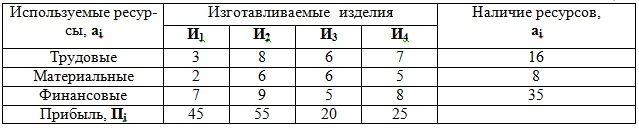
\includegraphics[width=1.\linewidth]{table.jpg}}  \\
\end{minipage}
\end{center}
\end{figure}
\newpage

{\bf3. Введение}

Профессиональная деятельность инженеров и ученых тесно связана с рассчетами, включающими в себя широкий спектр алгоритмов из различных разделов математики. Ввиду непрагматичности и затратности по времени и ресурсам самостоятельного создания алгоритмов на различных языках программирования, для рассчетов используются специализированные на этом математические пакеты и системы компьютерной алгебры, среди них: MatLab, MathCad, SciLab, SMath, Reduce и другие. Подобный подход позволяет работать с математическими алгоритмами в подготовленной среде с удобным интерфейсом без необходимости на затрату времени на создание кода с нуля. 

\newpage
{\bf4. Исследование функции}\\
1. Даны функции $f(x)=\sqrt{3}sin(x)+cos(x),g(x)=cos(2x+\frac{\pi}{3})-1$\\
а)Решить уравнение f(x)=g(x).\\
б)Исследовать функцию h(x)=f(x)-g(x) на промежутке $[0;\frac{5\pi}{6}]$\\
{\bfРешение уравнения.}\\
Задача а) эквивалентна следующей - требуется найти корни уравнения:\\
$h(x)=\sqrt{3}sin(x)+cos(x)-cos(2x+\frac{\pi}{3})-1$\\
Использование математических пакетов позволяет решать нелинейные уравнения двумя как численно, так и аналитически. Стандартный функционал SciLab позволяет нам получить численное решение, но к сожалению, не способен решить уравнение аналитически напрямую, поэтому для получения второго варианта решения нам придется воспользоваться системой компьютерной алгебры - Reduce.\\
{\bfЧисленное решение с применением SciLab.}\\
При отыскании решения воспользуемся стандартной функцией SciLab - fsolve.\\
Функция h(x), будучи линейной комбинацией периодических функций, обладает периодом равным наименьшему общему кратному периоду этих функций -- $2\pi$. Следовательно, для нахождения периодического решения нелинейного уравнения достаточно будет отыскать корни на отрезке $[0; 2\pi]$. \\
Решение функции fsolve основано на методе касательных и требует заданного интервала или начальной точки для поиска корней уравнения. Для нахождения начальных точек воспользуемся командой plot и построим график функции h(x) на данном отрезке:\\
function y=h(x)\\
y=sqrt(3)*sin(x)+cos(x)-cos(2*x+\%pi/3)+1\\
endfunction\\
plot(0:0.01:2*\%pi,h)\\
График функции отображен на Рис.1.
\newpage
\begin{figure}[H]
\begin{center}
\begin{minipage}[h]{0.65\linewidth}
\center{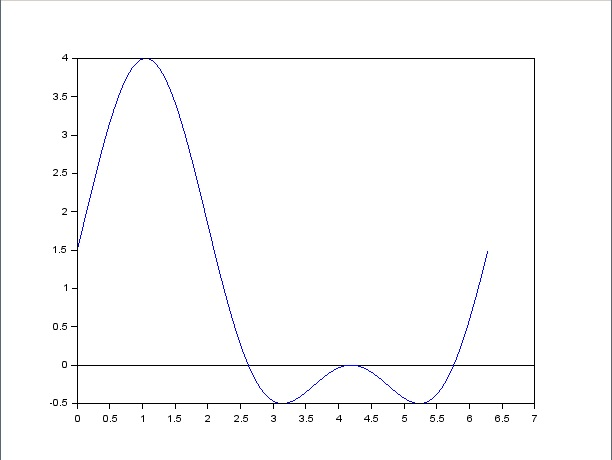
\includegraphics[width=1\linewidth]{scilab_1st.jpg}}  \\
\frametitle{ Рис 1. График функции h(x)}
\end{minipage}
\end{center}
\end{figure}

Отталкиваясь от от вида графика можно сделать предположение о наличии трех, либо четырех корней, при условии что график дважды пересекает ноль в промежутке x=[4.1;4.3].\\
Воспользуемся функцией fsolve для нахождения точек на графике:\\
$[x,v] = fsolve(x0,f)$, где:\\
x0 – вектор начальных значений для итеративного алгоритма отыскания нулей\\
f – функция, для которой осуществляется поиск нулей\\
x – вектор нулей функции, полученных при работе алгоритма из точек x0\\
v – вектор значений функции в точках x\\
Для проверки предположения о двойном пересечении графиком нуля в промежутке x=[4.1;4.3], укажем две начальных точки поиска с разных сторон от локального максимума, находящегося около x=4.2\\
Строки кода:\\
x0 = [3,3.9,4.5,5.5];\\
$[x,v] = fsolve(x0,h)$\\
v =\\
-2.220D-16 0. 0. 7.772D-16\\
x =\\
2.6179939 {\bf4.1887902} {\bf4.1887902} 5.759865

Полученные точки изображены на Рис.2.
\begin{figure}[H]
\begin{center}
\begin{minipage}[h]{0.65\linewidth}
\center{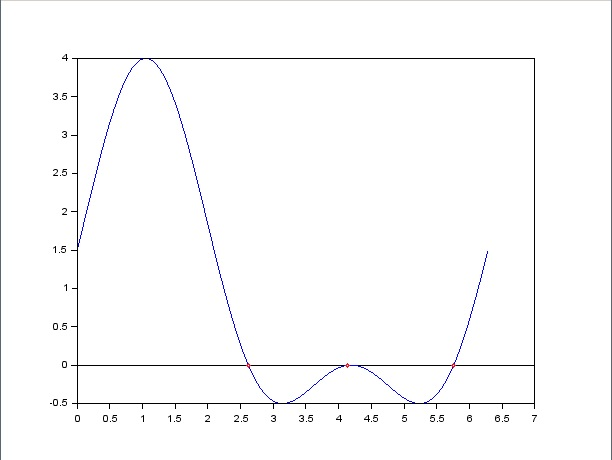
\includegraphics[width=1\linewidth]{scilab_2st.jpg}}  \\
\frametitle{Рис 2. График функции h(x) с корнями}
\end{minipage}
\end{center}
\end{figure}
\\
Согласно полученным значениям v, два решения не являются нулевыми, ввиду наличия определенной погрешности при решении с применением  fsolve. Также мы убедились, что функция не имеет четвертого корня на заданном отрезке.\\

Корни уравнения имеют следующий вид:\\
$$x_1=2.6179939+2n\pi,n\inZ$$
$$x_2=4.1887902+2n\pi,n\inZ$$
$$x_3=5.759865+2n\pi,n\inZ$$

Принимая во внимание тот факт, что корни линейной комбинации функций sin и cos могут быть кратны $\pi$, разделим полученные корни на данное значение:

x/\%pi =
0.8333333 1.3333333 1.3333333 1.8333333
Полученные десятичные дроби, как видно, кратны 1/3:
3*x/\%pi =
\\2.5 4. 4. 5.5
\newpage
В таком случае, корни приводятся к следующему виду:
$$x_1=\frac{5}{6}*\pi+2n\pi,n\in Z$$
$$x_2=\frac{8}{6}*\pi+2n\pi,n\in Z$$
$$x_3=\frac{11}{6}*\pi+2n\pi,n\in Z$$
Таким образом, используя несложные манипуляции мы перешли от численного решения к аналитическому.\\
\\
{\bfАналитическое решение с применением Reduce.}\\

Для нахождения аналитического решения уравнения воспользуемся функцией solve из системы компьютерной алгебры Reduce:\\
solve(expr,var); где\\
expr – система уравнений\\
var – список из переменных, относительно которых решаются уравнения expr\\

При попытке решить уравнение h(x)= 0 относительно x:\\
solve(sqrt(3)sin(x)+cos(x)-cos(2x+pi/3)-1,x);\\
Решение получено не было.\\
Упростим данное уравнение, воспользовавшись двумя тригонометрическими тождествами: $$sin(x+y)=sin(x)cos(y)+cos(x)sin(y)$$
$$cos(2x)=1-2sin^2(x)$$
$$\sqrt{3}sin(x)+cos(x),g(x)-cos(2x+\frac{\pi}{3})+1$$ $$=2(sin(x)cos(\frac{\pi}{6})+cos(x)sin(\frac{\pi}{6}))+2sin^2(x+\frac{\pi}{6})$$ $$=2(sin(x+\frac{\pi}{6})+sin^2(x+\frac{\pi}{6})$$\\
и получим упрощенное уравнение, эквивалентное исходному
$$2(sin(x+\frac{\pi}{6})+sin^2(x+\frac{\pi}{6})=0$$
Применим к нему функцию solve:\\
solve(2sin(x+pi/6)*(1+sin(x+pi/6)));
и получим решение:
\newpage

\begin{figure}[H]
\begin{center}
\begin{minipage}[h]{0.65\linewidth}
\center{{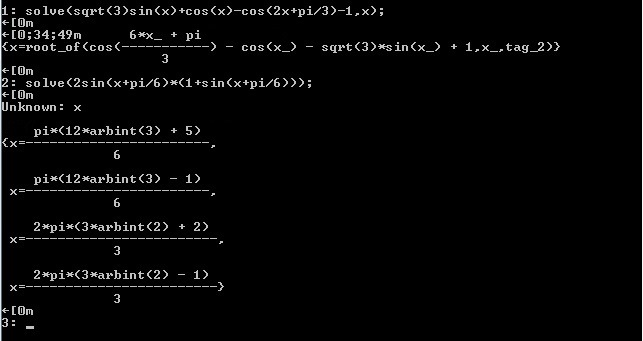
\includegraphics[width=1\linewidth]{reduce.jpg}\\
\frametitle{Ход решения уравнения с помощью Reduce}}}
\end{minipage}
\end{center}
\end{figure}


Где arbint является произвольным целым числом. Перепишем решение в более привычную для нас форму:

$$x_1=\frac{5}{6}*\pi+2n\pi,n\in Z$$
$$x_2=-\frac{1}{6}*\pi+2n\pi,n\in Z$$
$$x_3=\frac{8}{6}*\pi+2n\pi,n\in Z$$
$$x_4=-\frac{4}{6}*\pi+2n\pi,n\in Z$$\\
Периодические решения для $x_3$ и $x_4$совпадают, а периодическое решение для $x_2$ можно записать в виде:
$$x_2=\frac{11}{6}*\pi+2n\pi,n\in Z$$\\
Таким образом, с приненением двух различных математических пакетов и различных подходов были найдены корни нелинейной функции.

\newpage
{\bfИсследование функции на заданном промежутке.}\\
Исследуем функцию h(x) на промежутке $[0,5\frac{\pi}{6}]$.
Эта задача была частично выполнена в предыдущем разделе, где мы выяснили, что на заданном отрезке функция имеет ровно один корень в точке $x=5\frac{\pi}{6}$.\\
Продолжим исследование функции с использованием Reduce, как более располагающего к аналитическому изучению функции и её производных. Для начала определим функцию h в уже упрощенном виде:\\
h(x):=2sin(x+pi/6)*(1+sin(x+pi/6));
Определим значение функции на концах отрезка с помощью оператора подстановки sub:
sub(exp,f)=g, где\\
g-результат, полученный при подстановке списка алгебраических выражений в функцию.\\
Подстановка выражения вида x=const в функцию, зависящую только от аргумента x,равносильна её вычислению в этой точке.\\
В таком случае:\\
sub(x=0,h1)=3/2\\
sub(x=5pi/6,h2)=0\\
Отыщем первую и вторую производную аналитически с помощью оператора df:\\
df(f,x,n)=dif, где\\
dif – аналитическая форма производной n-го порядка для функции f по переменной x.\\
Определим в пространстве имен производные 1-го и 2-го порядка и выведем их:\\
dh1:=df(h,x,h1);\\
dh1:=df(h,x,h2);\\
plot(dh1,x=(0..5pi/6));\\
plot(dh2,x=(0..5pi/6));\\
\begin{figure}[H]
\begin{center}
\begin{minipage}[h]{0.77\linewidth}
\center{{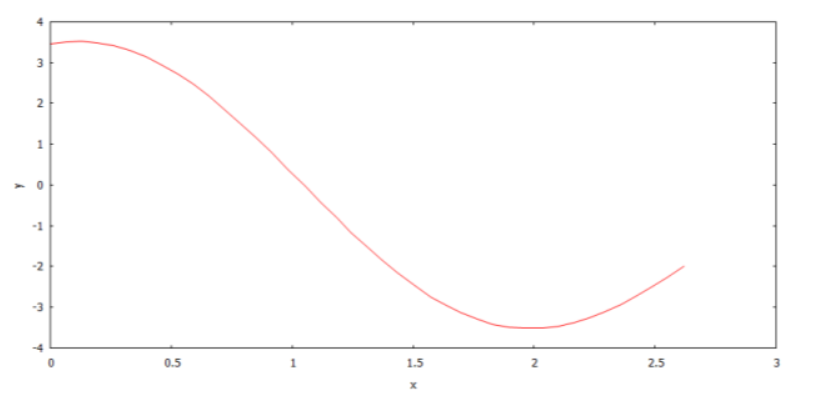
\includegraphics[width=1\linewidth]{function1.jpg}\\
\frametitle{График первой производной}}}
\end{minipage}
\end{center}
\end{figure}
\begin{figure}[H]
\begin{center}
\begin{minipage}[h]{0.75\linewidth}
\center{{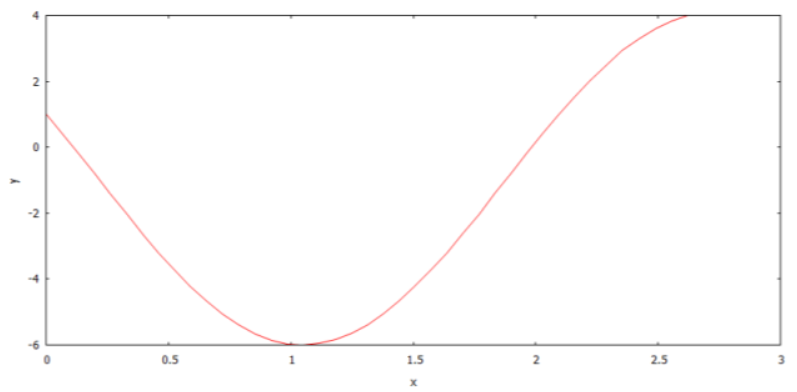
\includegraphics[width=1\linewidth]{function2.jpg}\\
\frametitle{График второй производной}}}
\end{minipage}
\end{center}
\end{figure}
Отыщем аналитически нули 1-ой и 2-ой производной, используя оператор solve:\\
solve(dh1,x);\\
solve(dh2,x);\\
\\
\newpage
\\
$\left\{x=\frac{\pi(6arbint(15)-1)}{3}, x=\pi(2arbint(15)+1), x=\frac{\pi(6arbint(14)+1)}{3}\right.$,\\ $\left.x=\frac{2\pi(3arbint(14)-1)}{3}\right\}$
\\
\\
$\left\{x=\frac{12arbing(16)\pi+12arctan(\frac{2\sqrt{-\sqrt{33}+9}}{4\sqrt{2}}-\sqrt{66}+\sqrt{2})-\pi}{6}\right.$,\\
$x=\frac{12arbing(16)\pi-12arctan(\frac{2\sqrt{-\sqrt{33}+9}}{4\sqrt{2}}+\sqrt{66}-\sqrt{2})-\pi}{6}$,$x=\frac{12arbing(16)\pi-12arctan(\frac{2\sqrt{-\sqrt{33}+9}}{4\sqrt{2}}-\sqrt{66}-\sqrt{2})-\pi}{6}$,\\
$\left.x=\frac{12arbing(16)\pi+12arctan(\frac{2\sqrt{-\sqrt{33}+9}}{4\sqrt{2}}+\sqrt{66}+\sqrt{2})-\pi}{6}\right\}$\\
\\
Из периодического решения для 1-ой произодной только $x=\frac{\pi}{3}$ находится на отрезке, на котором исследуется функция. Значит, на данном отрезке 1-ая производная имеет только один ноль.\\
Для упрощения аналитической формы 2-ой производной воспользуемся оператором нахождения численного решения num\_solve:\\
num\_solve(f,x = const) = f0, где\\
f0 – ноль функции f, найденный численно при начальной точке работы алгоритма x=const.\\
В качестве начальных точек алгоритма, отталкиваясь от вида графика 2-ой производной, зададим x=0.2 и x=2.4:\\
num\_solve(dh2,x=0.2)=0.111\\
num\_solve(dh2,x=2.4)=1.983\\

Отталикаясь от полученных результатов, можно сделать вывод, что функция:
1) Возрастает на промежутке (0,$\frac{\pi}{3}$)\\
2) Убывает на промежутке ($\frac{\pi}{3},5\frac{\pi}{6}$)\\
3) Имеет глобальный максимум в точке $x=\frac{\pi}{3}$\\
4) Имеет глобальный минимум в точке $x=5\frac{\pi}{6}$\\
5) Точки перегиба x=0.111 и x=1.193\\
6) Выпукла вверх на (0,0.111)U(1.193,$5\frac{\pi}{6}$)\\
7) Выпукла вниз на (0.111,1.193)\\
\newpage
{\bf5. Исследование кубического сплайна.}\\
Найти коэффициенты кубического сплайна, интерполирующего данные, представленные в векторах:\\
$V_x=[0,0.5,1.4,2.25,3.5]$\\
$V_y=[4,3.7,4.575,4.333,4.167]$\\
 Найти коэффициенты кубического сплайна, интерполирующего данные, представленные в векторах Vx и Vy.\\
Построить на одном графике: функцию f(x) и функцию f1(x), полученную после нахождения коэффициентов кубического сплайна.\\
Представить графическое изображение результатов интерполяции исходных данных различными методами с использованием встроенных функций cspline(Vx,Vy), pspline(Vx,Vy), lspline(Vx,Vy) и interp(Vk,Vx,Vy,x).\\
 Оценить погрешность интерполяции в точке x=2.4 и вычислить значение функции в точке x=1.4.\\
{\bf Нахождение коэффициентов кубического сплайна.}\\
Найдем коэффициенты кубического сплайна. Получив численное значение производных в точках с помощью функции splin, отыщем 4 решения для системы линейных уравнений (в соответствии с количеством узлов), в которых переменными и являются коэффициенты:
$A_i*сf_i=Y_i$\\
i=0,...,4-индекс интервала\\
$A_i=$
\begin{bmatrix}
1&x_i&x^2_i&x^3_i\\
1&x_i_+_1&x_i_+_1^2&x_i_+_1^2\\
0&1&2x_i&3x^2_i\\
0&1&2x_i_+_1&3x_i_+_1^2\\
\end{bmatrix}\\
$Y_i=(y_i,y_i_+_1,d_i,d_i_+_1)^T$\\
$x_i$-узлы интерполяции\\
$y_i$-значение функции в узлах интерполяции\\
$d_i$-значение производной в углах интерполяции\\
$сf_i$-коэффициенты i-го кубического сплайна
\newpage
$сf_i=A_i^-1*Y_i$\\
Код соответствующий решению уравнений (выбранное граничное условие – равенство третьих производных слева и справа для точек $x_2$ и $x_3$):\\
$x = [0,1.25,2,2.625,4.25];\\
y = [2,1.925,2.4,2.7,3.64];\\
d = splin(x,y);\\
n = length(x)-1;\\
cfs = zeros(4,n);\\
for i = 1:4\\
    a = x(i);\\
    b = x(i+1);\\
cfs(:,i) = [1,a,a^2,a^3; 1,b,b^2,b^3; 0,1,2*a,3*a^2; 0,1,2*b,3*b^2]/ [y(i);y(i+1);d(i);d(i+1)]\\$
end\\
cfs =\\
$\begin{bmatrix}
4.&4.&-0.4828416&-0.4828416\\
-1.9441828&-1.9441828&7.6619065&7.6619065\\
3.247419&3.247419&-3.6140733&-3.6140733\\
-1.1181069&-1.1181069&0.5155817&0.5155817\\
\end{bmatrix}\\$
 Построим график интерполянта и интерполянта на линейных сплайнах:\\
$for i=1:4\\
t = linspace(x(i),x(i+1));\\
plot(t,interpln([x;y],t));\\
plot(t,cfs(:,i)'*[ones(t); t; t.^2; t.^3]);\\$
end
\newpage
\begin{figure}[H]
\begin{center}
\begin{minipage}[h]{0.70\linewidth}
\center{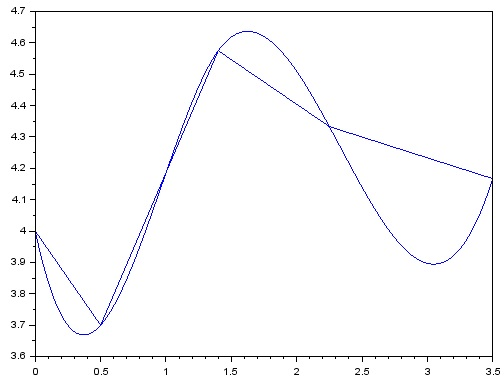
\includegraphics[width=1\linewidth]{spline.jpg}}  \\
\frametitle{Рис. 3. График интерполянянтов, полученных из коэффициентов кубических сплайнов и из линейных сплайнов}
\end{minipage}
\end{center}
\end{figure}
Найдем значение в точке x=1.4, с использованием интерполяции полинома в точке x, а так же погрешность в точке x=2.4, с помощью абсолютной разницы между интерполяциями линейного и кубического сплайна:\\
X=[1.4];\\
Y=interp(X,x,y,d);\\
Y=4.575\\
\\
Xe=[2.4];\\
Ye=interp(Xe,x,y,d);\\
Yl=interpln([x;y],Xe);\\
Er=abs(Yl-Ye)\\
Er=0.09700644947016812\\
\newpage
{\bfИнтерполяция встроенными методами.}\\
В SciLab интерполяцию можно произвести воспользовавшись следующими двумя командами:\\
d=splin(x,y,”параметр”);\\
is=interp(xx,x,y,d);\\
Где $x=[x_1,x_1,...,x_n_-_1,x_1]$\\
y – значения функции в узлах интерполяции\\
is – значения интерполянта (кубического сплайна, интерполирующего заданную функцию) вычисленные в точках x.\\
”параметр” – параметр, отвечающий за граничное условие интерполянта\\
Условия, соответствющие различным параметрам:\\
1)”natural” - производные в точках x1,xn, интерполянты равны нулю\\
2)”clamped” - точное задание производных в точках $x_1,x_n$\\
3)”not\_a\_knot” - 3-я производная слева и справа равны для точек $x_2$,$x_n_-_1$\\
4)”fast” – расчет сплайна на основе обычной интерполяции кубическим полиномом\\
5)”monotone” – на интервалах между узлами интерполянт является монотонным\\
Для построения графиков интерполянтов с различными граничными условиями воспользуемся следующими командами:\\
x=[0,0.5,1.4,2.25,3.5];\\
y=[4,3.7,4.575,4.333,4.167];\\
t=0:0.01:4.575;\\
xx=[0;0];\\
plot2d(t,interp(t,x,y,splin(x,y,"natural")))\\
plot2d(t,interp(t,x,y,splin(x,y,"clamped",xx)))\\
plot2d(t,interp(t,x,y,splin(x,y,"not-a-knot")))\\
plot2d(t,interp(t,x,y,splin(x,y,"fast")))\\
plot2d(t,interp(t,x,y,splin(x,y,"monotone")))\\
\newpage
\begin{figure}[H]
\begin{center}
\begin{minipage}[h]{0.70\linewidth}
\center{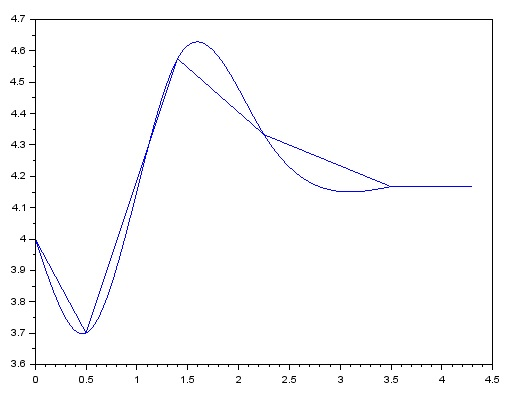
\includegraphics[width=1\linewidth]{natural.jpg}}  \\
\frametitle{Рис 4. Интерполянт splin(,,”natural”)}
\end{minipage}
\end{center}
\end{figure}
\begin{figure}[H]
\begin{center}
\begin{minipage}[h]{0.70\linewidth}
\center{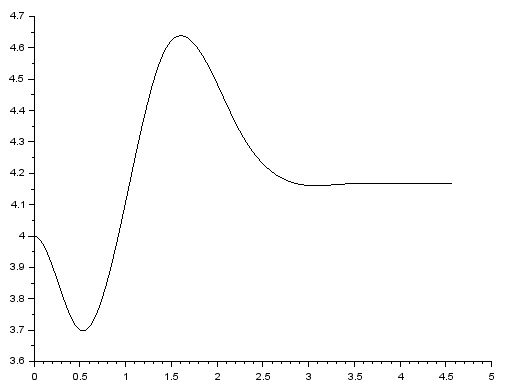
\includegraphics[width=1\linewidth]{clamped.jpg}}  \\
\frametitle{Рис 5. Интерполянт splin(,,”clamped”)}
\end{minipage}
\end{center}
\end{figure}
\begin{figure}[H]
\begin{center}
\begin{minipage}[h]{0.70\linewidth}
\center{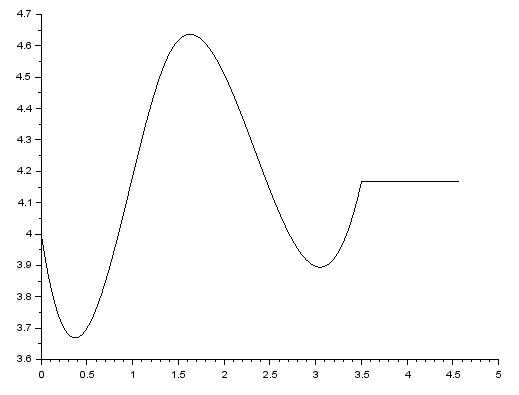
\includegraphics[width=1\linewidth]{not_a_knot.jpg}}  \\
\frametitle{Рис 6. Интерполянт, полученный с помощью splin(,,”not-a-knot”)}
\end{minipage}
\end{center}
\end{figure}
\begin{figure}[H]
\begin{center}
\begin{minipage}[h]{0.65\linewidth}
\center{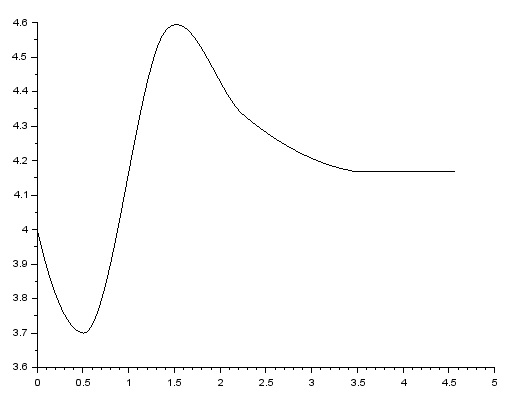
\includegraphics[width=1\linewidth]{fast.jpg}}  \\
\frametitle{Рис 8. Интерполянт, полученный с помощью splin(,,”fast”)}
\end{minipage}
\end{center}
\end{figure}
\begin{figure}[H]
\begin{center}
\begin{minipage}[h]{0.65\linewidth}
\center{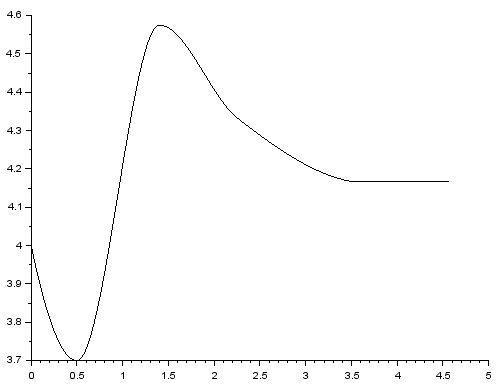
\includegraphics[width=1\linewidth]{monotone.jpg}}  \\
\frametitle{Рис 9. Интерполянт, полученный с помощью splin(,,”monotone”)}
\end{minipage}
\end{center}
\end{figure}

{\bf6. Задача оптимального распределения неоднородных ресурсов.}\\
Требуется решить следующую задачу оптимального распределения неоднородных ресурсов: Для изготовления {\bf n} видов изделий {\bfИ$_1$}, {\bfИ$_2$} ,... , {\bfИ$_n$} необхо¬димы ресурсы m видов: трудовые, материальные, финансовые и др. Известно тре¬буемое количество отдельного i-гo ресурса для изготовления каждого j-го изделия. Назовем эту величину нормой расхода {\bf C$_i_j$}. Пусть определено количество каждого вида ресурса, которым предприятие располагает в данный момент, - {\bf a$_i$}. Известна прибыль {\bfП$_j$}, получаемая предприятием от изготовления каждого j-го изделия. Требуется определить, какие изделия и в каком количестве должны производиться предприятием, чтобы прибыль была максимальной.  \\
Исходные данные:\\
\begin{figure}[H]
\begin{center}
\begin{minipage}[h]{0.75\linewidth}
\center{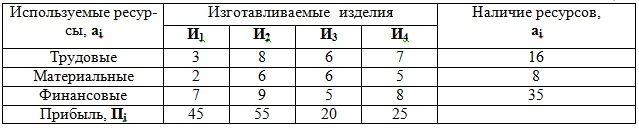
\includegraphics[width=1.\linewidth]{table.jpg}}  \\
\end{minipage}
\end{center}
\end{figure}

Для решения данной задачи, являющейся задачей линейного программирования, мы воспользуемся командой linpro из пакета quapro для SciLab, специально предназначенной для решения задач линейного программирования и хорошо адаптированная под решение данной задачи оптимизации.\\

Общий вид решения:\\
$[x,lagr,f]=linpro(-p,C,b,ci,cs);$\\
\\
где p – массив(вектор-столбец) коэффициентов при неизвестных целевой функции, длина вектора n совпадает с количеством неизвестных x. Так как по условию задачи нужно найти максимум функции, то параметр p возьмем со знаком «-».\\
C – матрица при неизвестных из левой части системы ограничений, количество строк матрицы равно количеству ограничений, а количество столбцов совпадает с количеством неизвестных.\\
b – массив (вектор-столбец), содержит свободные члены системы ограничений.\\
ci - массив (вектор-столбец) содержит нижнюю границу переменных (cij ≤ xj); если таковая отсутствует, указывают [ ].\\
cs - массив (вектор-столбец) содержит верхнюю границу переменных (csj ≥ xj); если таковая отсутствует, указывают [ ].\\
\\
Зададим значения переменных функции в соответствии с таблицей исходных данных:\\
p=[45;55;20;25];\\
C=[3,8,6,7;2,6,6,5;7,9,5,8];\\
b=[16;8;35];\\
ci=[0;0;0;0];\\
cs=[];\\
\\
\newpage
Произведем поиск решения:\\
$[x,lagr,f]=linpro(-p,C,b,ci,cs);$\\
\\
f  =\\
  - 180  // Максимальная прибыль\\
 larg  =\\
    0.   \\  
  - 80.   \\
  - 155.\\
  - 87.5   \\
    0.   \\
    22.5   \\
    0.     \\
 x  =		// Объем производства\\
    4. \\
    0.    \\
    0.    \\
    0. \\
\\
Таким образом, искомым целочисленным решением доставляющим максимум целевой функции является вектор [4;0;0;0], а значением целевой функции, отвечающему этому вектору, - 180. Иными словами, для получения прибыли в 180 у.е. потребуется произвести 4 единицы первого изделия.
\\
\\
{\bf 7. Выводы}\\
В ходе выполнения курсовой работы были изучены методы практического применения встроенных функций математического пакета SciLab и системы компьютерной алгебры Reduce, а так же их надстроек. Был произведен поиск нулей функции, ее аналитическое исследование, интерполяция функции кубическими сплайнами, линейное программирование.
\end {document}
